\section{User interface}
User interface består overordnede af en skærm og 2 knapper. En knap til at start og stoppe funktioner og en knap til at måle blodtryk. Til brugerfeedback er der en display hvorpå trykket, patient ID, resterende tid og antallet af gennemførte cyklusser vises. Apparatet betjenes i tre forskellige stadier “Konditionering, Okklusion og setup”. Disse tre stadier er beskrevet med hver siden illustration nedenfor. For at skifte mellem disse stadier er der en mode switch på bagsiden af apparatet, den er også beskrevet nedenfor: 

\subsection{Konditionering}
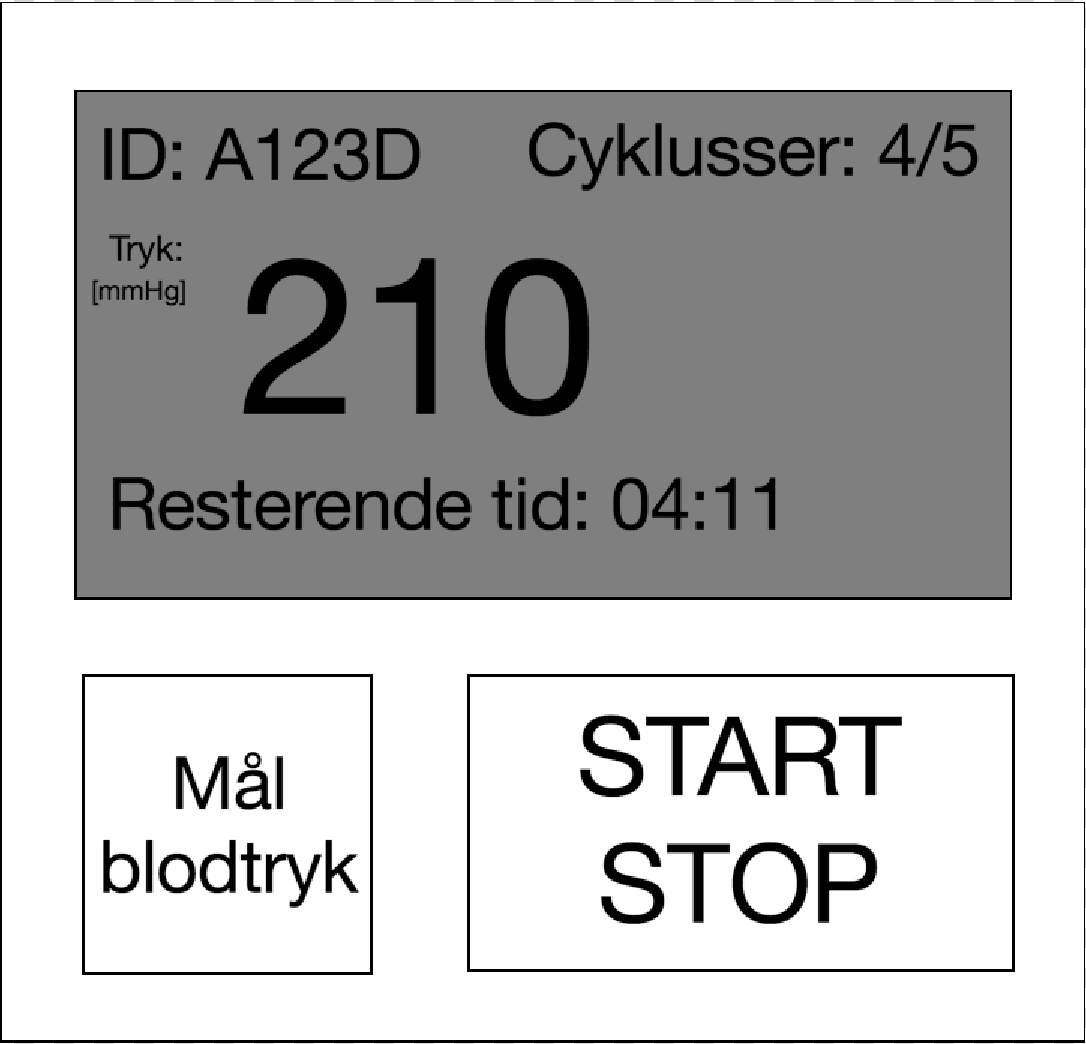
\includegraphics[width=\textwidth]{KonditioneringGUI}
\subsection{Okklusion}
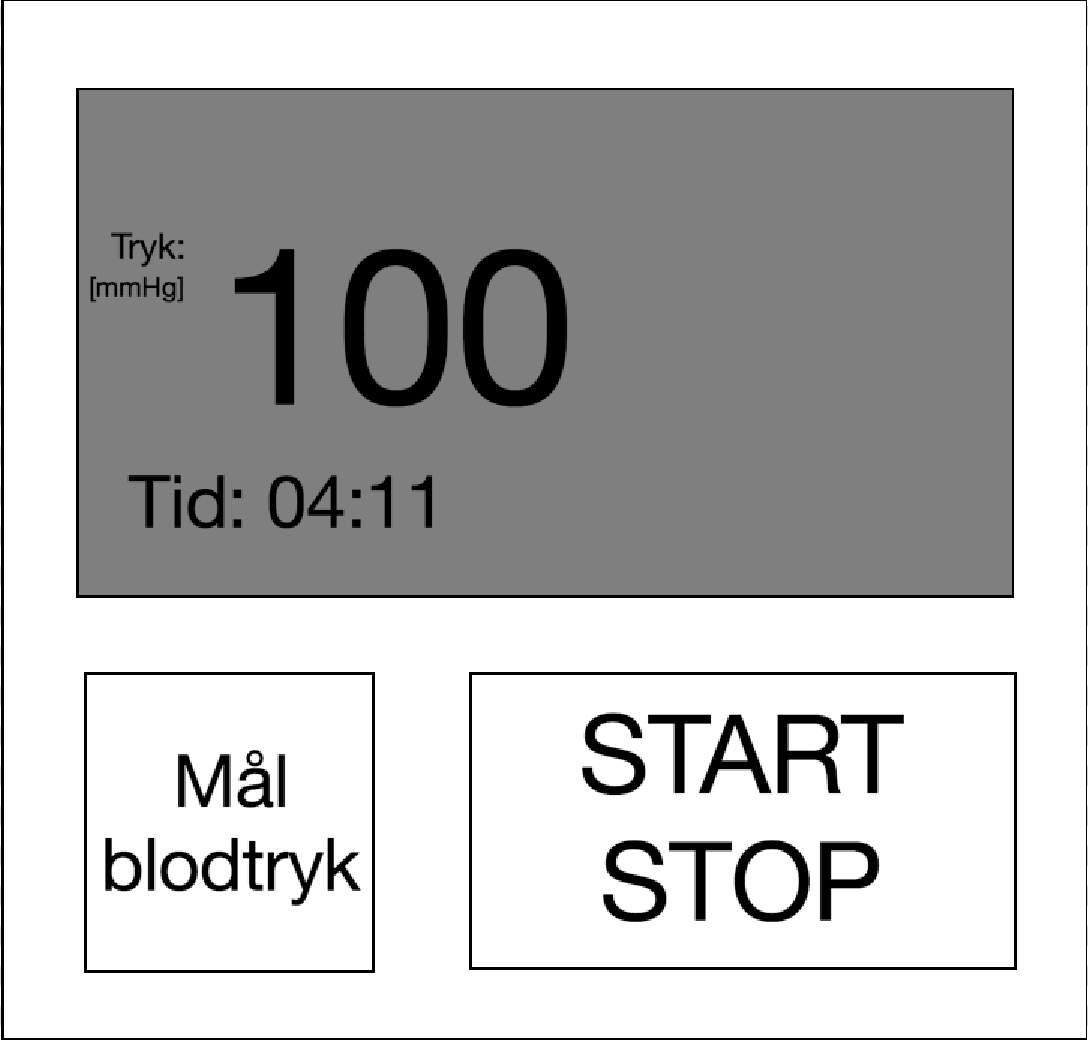
\includegraphics[width=\textwidth]{OkklusionGUI}

\subsection{Setup}
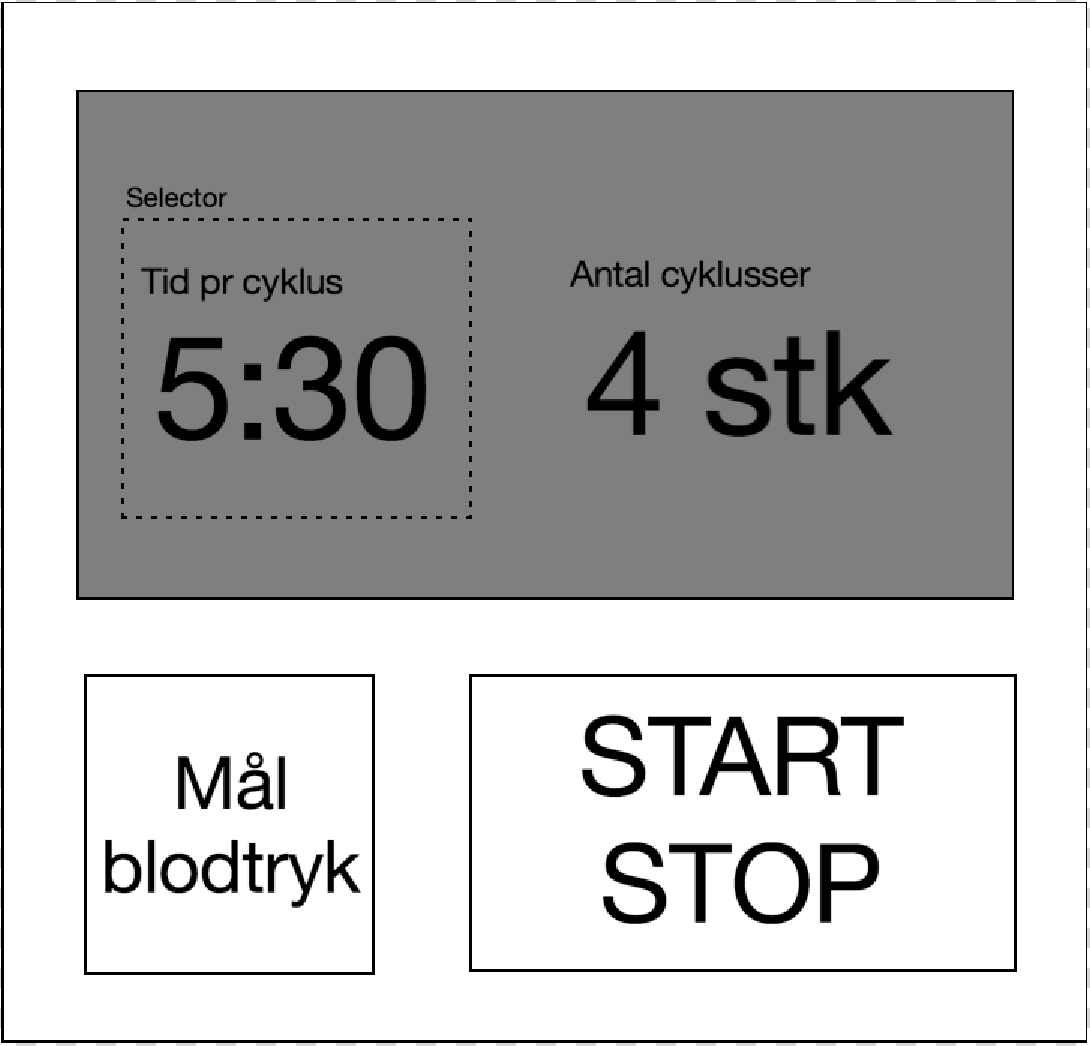
\includegraphics[width=\textwidth]{SetupGUI}

\subsection{Bagside}
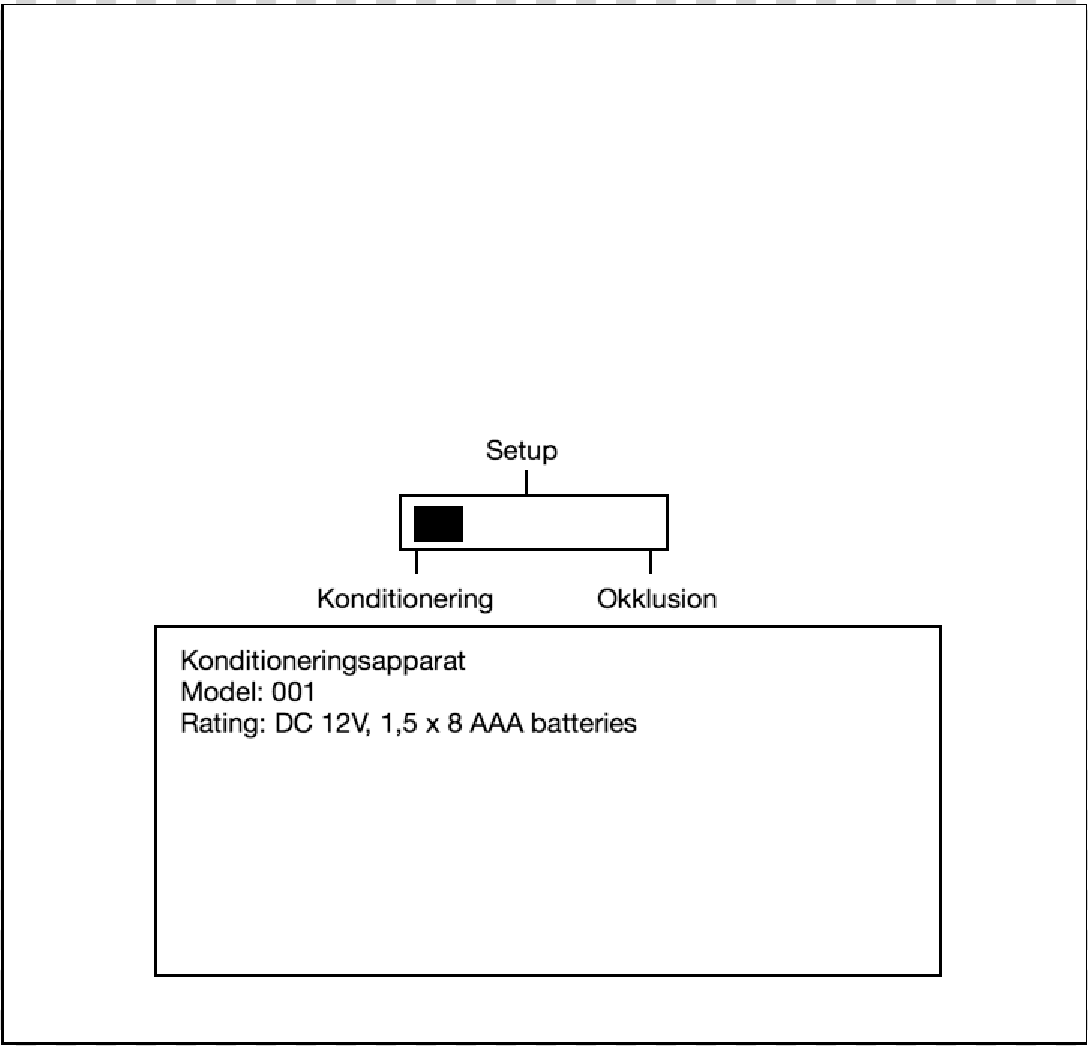
\includegraphics[width=\textwidth]{BagsideGUI}
